\chapter{Elemento Spring}

\section{Fundamento teórico}

El elemento \textit{Spring} (resorte) es un elemento finito unidimensional donde 
las coordenadas locales y globales coinciden. Cada elemento spring tiene dos 
nodos como se muestra en la figura \ref{fig:spring_element}. Sea la rigidez del 
resorte la denotada por $k$, en este caso la matriz de rigidez del elemento está 
dada por:

\begin{equation}
K_{(e)} = \begin{bmatrix}
k & -k \\
-k & k 
\end{bmatrix}
\end{equation}

\begin{center}
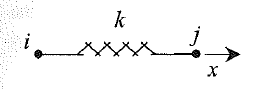
\includegraphics[scale=0.8]{src/spring-element/spring_element.png}
\captionof{figure}{Elemento spring}
\label{fig:spring_element}
\end{center}

Obviamente la matriz de rigidez para un elemento \textit{spring} es de $2\,x\,2$, dado que 
este tiene dos grados de libertada, uno en cada nodo. Consecuentemente para un 
sistema de elementos \textit{spring} con $n$ nodos, el tamaño de la matriz global de 
rigidez $K$ será de $n\,x\,n$. La matriz global de rigidez se obtiene ensamblando 
los matrices de rigidez por elemento $K_{(i)}$ para $i=1,2,...,n$, utilizando el método 
directo de la rigidez.\\

Una vez que la matriz global de rigidez $K$ es obtenida  se tiene un sistema de ecuaciones 
de la forma:

\begin{equation}
[K]\{U\} = \{F\}
\end{equation}

Donde $U$ es el vector global de desplazamientos nodales y $F$ es el vector global de 
fuerzas nodales.\\

El sistema de ecuaciones resultantes se puede simplificar aplicando las condiciones 
de frontera o restricciones de desplazamiento, quedando generalmente un sistema 
de menor dimensión el cuál está determinado y puede resolverse utilizando métodos 
de álgebra lineal´, quedando una posible solución como:

\begin{equation}
\overline{U} = \overline{K}^{-1}\, \overline{F}
\end{equation}

Donde $\overline{U}, \overline{K} \,\, y \,\, \overline{F}$ corresponden a las variables descritas 
anteriormente, después de aplicar las condiciones de frontera correspondientes.


\section{Un ejemplo resuelto en NuSA}

En lo subsecuente se propone un ejercicio de elementos \textit{spring} y se resuelve 
utilizando la librería NuSA.

\textbf{Ejemplo 1.} Para el ensamble mostrado en la figura \ref{fig:example_01}, calcular 
a) la matriz global de rigidez  b) los desplazamientos de los nodos 3 y 4  c) las fuerzas 
de reacción en los nodos 1 y 2, y  d) las fuerzas en cada elemento. Una fuerza de 5000 lb 
es aplicada en el nodo 4 en la dirección $x$, las constantes de rigidez para cada resorte 
se muestran en la figura. Los nodos 1 y 2 están fijos.

\begin{center}
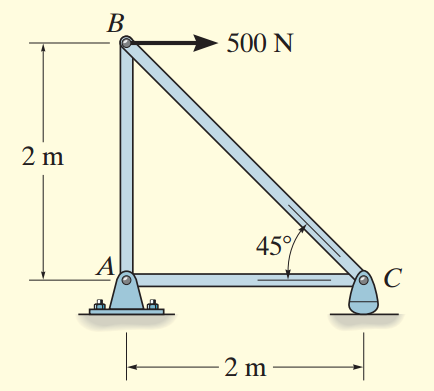
\includegraphics[scale=0.8]{src/spring-element/example_01.png}
\captionof{figure}{}
\label{fig:example_01}
\end{center}

